\documentclass{ctexart}
\setCJKmainfont{BabelStone Han}
\usepackage{CJKutf8}
\renewcommand{\figurename}{圖}
\usepackage{natbib}
\RequirePackage{filecontents}
\usepackage{url}
\usepackage{natbib}
\usepackage{graphicx}
\usepackage{minted}
\usepackage{booktabs}
\usepackage[a4paper, margin=1.5cm]{geometry}

\begin{filecontents}{\jobname.bib}
@misc{linux programmer's manual, url={https://man.archlinux.org/man/fcntl.2.en#Mandatory_locking}, journal={Linux Programmer's Manual}} 
\end{filecontents}
\begin{document}
\pagestyle{headings}
\title{系統程式 作業03}
\author{409410005 鍾天睿}
\date{March 20 2021}
\maketitle
\clearpage

\section{系統環境}
\begin{center}
\begin{tabular}{ l l } 
\hline
發行版 & Arch Linux  \\
\hline
Linux Kernel & 5.10.16-arch1-1  \\
\hline
GCC 版本 & 10.2.0 \\
\hline
Clang 版本 & 11.1.0 \\
\hline
GDB 版本 & 10.1 \\
\hline
CPU & Intel i7-10510U \\
\hline
硬碟 & Samsung PM981 M.2 512 GB PCI Express 3.0 NVMe \\
\hline
\end{tabular}
\end{center}

\section{程式說明}
\subsection{安裝 \& 執行}
輸入指令 \mintinline{bash}{make run_flock} 以編譯及執行。
\section{利用 FLock 鎖定檔案}
程式 \mintinline{bash}{flock.c} 中使用 flock 鎖定檔案。程式內容為讀取 \mintinline{bash}{flock.db} 最後 2 bytes 的 unsigned short integer,並將游標往後 x bytes,再寫入下個數字。作業要求程式中迴圈執行 3000 次,執行 4 次程式,所以型態的部份選用 unsigned short 只佔2 bytes。
\subsection{檔案大小估計}
檔案內共有 $3000\times4=12000$ 個數字,共 24000 bytes。空白部份為 
$\sum _{n=3500}^{3500+12000}n = 113994004$ bytes。合計 113974000。硬碟最小區塊為 4k,但是看起來好像剛好可以整除。

\section{利用 LockF 鎖定檔案}
使用強制鎖鎖定
檔案需要 mount 時加上 \mintinline{bash}{mand} 選項,但是我所使用的發行版無法使用,掛載時候會出現 permission denied error (errno 32)。使用 \mintinline{bash}{journalctl -xe} 發現以下訊息:
\begin{minted}{bash}
kernel: VFS: "mand" mount option not supported
\end{minted}
根據 Linux 文件\footnote{\url{https://man.archlinux.org/man/fcntl.2.en#Mandatory_locking}},Linux 的強制鎖實現是不可靠的,應當避免使用。我使用的發行版沒將強制鎖預編譯至 kernel。
\clearpage
\section{實驗}
同時執行 4 個 flock.c 產生的檔案如下:
\begin{figure}
    \centering
    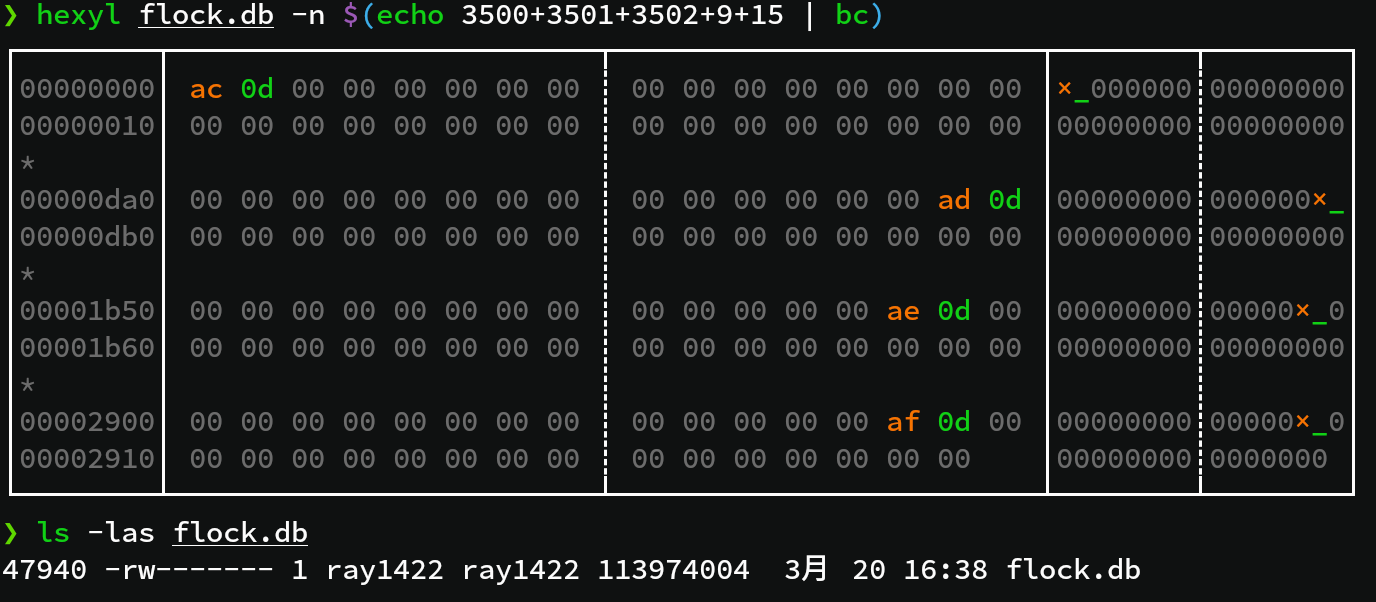
\includegraphics[width=\linewidth]{160649109_731735200844467_3217228969766850594_n.png}
    \caption{使用 hexyl 查看生成的檔案}
    \label{fig:my_label}
\end{figure}
使用 hexyl 檢視生成的 flock.db 檔案,第一個數值為 \mintinline{bash}{0x0DAC} (C 的unsigned short 後面為前面位數),換算後為 3500;最後一個數值是 15499,檔案大小也符合預期。
\section{結論}
使用 FLock 可以避免同時執行時,資源未經鎖定而造成的讀寫內容錯誤。
\end{document}
